We have used different ideas and methods in this project. In this chapter methods are explained in following 
\textit{\hyperref[mth:preproces]{Preprocessing}}, 
\textit{\hyperref[mth:wordrep]{Word Representation}}, 
\textit{\hyperref[mth:features]{Features}}, 
\textit{\hyperref[mth:ml]{Machine Learning}}, 
\textit{\hyperref[mth:balance]{Balancing}}, 
\textit{\hyperref[mth:dl]{Deep Learning}}, 
\textit{\hyperref[mth:a2c]{Article to Claim}}, and 
\textit{\hyperref[mth:fn]{Fake News Detection}} sections.

\section{Preprocessing}
\label{mth:preproces}
The first and mandatory preprocessing step is to tokenize words in the corpus in order to remove and detect special words. After tokenization, a list of punctuation and Persian stop-words are considered as \textit{denied} words and are removed from the corpus in this step. We chose stop-words carefully in a way not to lose refuting or supporting expressions in news context. Verbs carry valuable information to detect stance of an article. Nonverbal stop-word class is a better choice to remove low-value words in this task. Also English number characters will remove from the corpus before tokenizing. 

\section{Features}
\label{mth:features}
In machine learning algorithms, feature engineering can be considered the most important step because the desired model trains patterns only corresponding to predictors. Extracting sufficient predictors as compact as possible to having the best predicting accuracy and time-efficient	, requires numerous trials and errors. In the following part of this section, extracted features are explained in detail.

\subsection{Similarity}
The similarity score is offered by \cite{stance_persian}. This feature calculates how much a claim is similar to a headline or a news article, depends on the task. Three following sequence matching score is considered for this feature.

\begin{itemize}
	\item Ratio: Similarity score in float range 0,1. This parameters calculates from equation \ref{eq_ratio}
	\begin{equation}
		\label{eq_ratio}
		\text{ratio} = \frac{2.0 * M}{T}
	\end{equation}
	where:
	\begin{eqexpl}[25mm]
		\item{$T$}Number of elements in both sequences.
		\item{$M$}Number of matches.
	\end{eqexpl}
	\item Quick Ratio: This parameter estimates an upper bound on the Ratio.
	\item Real Quick Ratio: This parameter estimates an upper bound on the Ratio.
\end{itemize}

\subsection{Root Distance}
This feature is suggested by \cite{stance_persian}. Root Distance stands for the distance between the root of a headline and some collected hedge, refuting and reporting words. Firstly, a set of words considered as mentioned group are gathered, and then for each word distance is calculated.

\subsection{ImportantWords}
List of a controversial and challenging words in news gathered by \cite{stance_persian} and considered as \textit{important-words} in this project. This feature is a zero-based list with the length of important words, and each cell stands for one word in \textit{important-words}. The list carries the number of repetitions of desire words in a specific news article.
\subsection{Is Question}
Is-Question identifies whether a claim or headline of a news article ends with question marks or not. \cite{stance_persian} dataset contains a column dedicated to this feature.
\subsection{Has Two Parts}
Has-Two-Parts is if a claim is constructed of two separate parts. \cite{stance_persian} dataset contains a column dedicated to this feature.
\subsection{Polarity}  
The polarity of a text can be utilized in a variety of tasks. This feature presents how positive or negative a text is. Different algorithms are developed to predict the polarity of a text. In this project, \cite{persent} dataset is used to calculate each sample sentiment. \cite{persent} contains a dictionary of words with their sentiment score between -1 and 1. The more negative the word meaning, the lower its polarity point. For each word presents in each sample at most first 30 nonzero polarity value saves in a zero initialed vector with 30 lengths. As \cite{persent} contains only 1500 word polarity values, it can't cover all words in corpus and it has a far way to improve. 

In this project, an idea is applied to extend PerSent (\cite{persent}) polarity dataset is to use a language model. It is possible to predict similar words with a particular word and estimate their similarity score with a language model. Firstly, similar words that don't polarity score in PerSent with their similarity scores extract from a pre-trained language model. Then search each word in the PerSent dataset (\cite{persent}) and apply equation \ref{eq_polar} average through all similar words polarity scores, to estimate the desired word polarity score.

\begin{equation}
	\label{eq_polar}
	\text{polarity\_score}\left(w\right) = \frac{\Sigma_{w^{`} \in W} \text{Similatiry}\left(w^{`}, w\right) . \text{Polarity}\left(w^{`}\right)}{\Sigma_{w^{`} \in W} \text{Similatiry}\left(w^{`}, w\right)}
\end{equation}

where: 
\begin{eqexpl}[25mm]
	\item{$w$}Desire word $\notin$ PerSent datast.
	\item{$W$}Similar words, Predicted by the language model
	\item{$\text{Similarity}$}Similarity score for 2 words which is predicted by the language model.
	\item{$\text{polarity}$} Polaroty score which is estimated by \cite{persent} dataset.
\end{eqexpl}

\bigbreak
One alternative is to use a deep neural networks model to predict score polarity of a word whether word-level or sentence-level. But due to the lack of a Persian dataset in news context, it is not practical. Available datasets for sentiment analysis are mainly gathered from customer comments on special businesses. For instance \cite{polar_hotel} used 2 different datasets, first it translated English sentiment analysis corpus and second used comments on hotels. \cite{polar_servic} used dataset from SnappFood\footnote{snappfood.ir}, DigiKala\footnote{digikala.ir} comments. One main problem with these datasets is the different use of language between user comments and news. Users mostly use everyday language on the other hand news agencies use formal language.



\section{Balancing}
\label{mth:balance}
Balancing methods is needed to compensate lack of data in classes except the majority class. Imbalance datasets make models to be biased on the majority class and there may be not enough samples in other classes for a model to learn that. This leads to having high accuracy score (Equation \ref{eq:acc}) while having low f1 score (Equation \ref{eq:f1}). There are several algorithms to deal with imbalanced datasets. It's not practical to rely on only one method and except to perform in the best way. Consequently, three different methods are applied on to the dataset in order to deal with this phenomenon. Methods of balancing a dataset which is used in this project are described in the following sections.  
	
\subsection{Extending dataset}
The simplest method is to gather data for classes except for the majority class. But unfortunately, it is not always practicable. Another way of extending a dataset is to use another existing dataset which has similar gathering logic and it is possible to map these two dataset classes. 

ParsFEVER (\cite{parsfever}) is a Persian dataset set based on FEVER (\cite{fever}) dataset is gathered for fact extraction and verification task. \cite{parsfever} claims are generated from Wikipedia\footnote{wikipedia.org} articles manually, then pieces of evidence for each claim are extracted from Wikipedia separately by distinct annotators. This dataset contains three \textit{Support}, \textit{Refute}, and \textit{Not Enough Info} classes. 
\begin{itemize}
	\item {\color{green!70!black}\textbf{Support:}} The article obviously proves the given claim. 
	\item {\color{red!60!black}\textbf{Refute:}} The article obviously disproves the given claim.
	\item {\color{gray}\textbf{Not Enough Info:}} There isn't enough information in the article about the claim. 
\end{itemize}                

According to Figure \ref{fig:datacom} two \textit{Agree} and \textit{Disagree} class in \cite{stance_persian} dataset suffers from lack of samples. In this project, \textit{Supports} and \textit{Refutes} samples from \cite{parsfever} dataset are mapped to \textit{Agree} and \textit{Disagree} class of \cite{stance_persian} dataset respectively. 
But it is not possible to extend \textit{Discuss} or \textit{Unrelated} class by ParsFEVER, because they are both merged in \textit{Not Enough Info} class. As a result, two \textit{Agree} and \textit{Disagree} extended as much as possible with random selected samples from ParsFEVER dataset. Sample distribution is illustrated in figure \ref{fig:datab1}. Dataset is still imbalanced in one class for both Article to Claim and Headline to Claim.


\subsection{Oversampling and Undersampling}
 Desired oversampling methods to deal with imbalanced dataset are RandomOverSampler, SMOTE, SVMSMOTE, BorderlineSMOTE, and ADASYN which are described in section \ref{lr:oversampling}. 

\subsection{Tune mode parameters}
 The last but not least important balancing method is to choose a robust learning algorithm for an imbalanced dataset, Choosing a weight of each class according to the ratio of samples of each class and choosing an optimizer and loss function that can overcome an imbalanced dataset.

\section{Machine Learning}
\label{mth:ml}
Figure \ref{fig:mlschm} illustrates a basic schematic of each machine learning models. Input of the model are samples in the dataset. After prepossessing, then predictors extracts from Feature Extractor module. The description of each predictor described in detail at section \ref{mth:features}. As the next step, before feeding data into classifier modules, balancing dataset is performed on dataset training set. Finally, samples classify in to one of four desired labels. 
\begin{figure}% 
	\centering
	{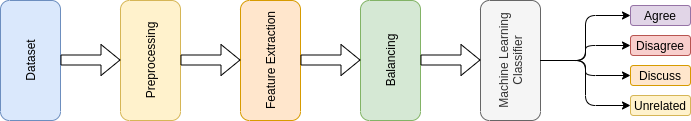
\includegraphics[width=14.5cm]{statistics/schema/ml.png} }
	\caption{Schematic of each machine learning model.}%
	\label{fig:mlschm}%
\end{figure}


\section{Deep Learning}
\label{mth:dl}
In the deep learning approach, a combination of all predictors can be fed into the model and the model on its own will automatically learn which predictor is useful for the task. This property is the biggest advance of deep learning in comparison to machine learning (\cite{book_datafake}). On the contrary, in machine learning, it was a critical step to design input predictors that the model can perform the best. And hours of trying different combination of predictors is needed (\cite{book_fake}). \cite{stance_robust} assessed that, In contrast, deep learning models, machine learning models that are trained on a single dataset, usually generalize poorly to other domains.

The schematic of the deep learning model is shown in figure \ref{fig:dlschm}. Headline-to-claim and Article-to-claim models have the same schematic. Only the input shape of parameters varies in each model. In comparison to Figure \ref{fig:mlschm} Feature Extraction is omitted from the machine learning model. Besides, the Deeplearning module constructs of pre-trained language model and a few Dense layers at its top. We evaluated BERT, ParsBERT, and ALBERT language models against each other in this project (More description in section \ref{lr:lm}).
\begin{figure}% 
	\centering
	{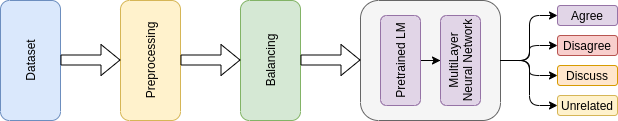
\includegraphics[width=14.5cm]{statistics/schema/dl.png} }
	\caption{Schematic of each deep learning model.}%
	\label{fig:dlschm}%
\end{figure}


\section{Article to Claim}
\label{mth:a2c}
Deep learning models perform far better on language inference tasks so they are better choices for article-to-claim stance classification. To calculate the stance of a claim toward the body of a news article, three different models based on a pre-trained Persian language model based on BERT, ParsBERT, and  ALBERT (More description in section \ref{lr:lm}) are evaluated against each other. 

\section{Fake News Detection}
\label{mth:fn}
	\label{sec:fakenews}
Schematic of fake news pipeline is shown in figure \ref{fig:fnschm}. To detect a news article's veracity, headline-to-claim and article-to-claim stance detection models, are considered as a black box. Four news articles are considered to evaluate the veracity of a claim. Firstly, the stance of a claim toward each headline of desired news articles and the body of the news article predict by stance classifier models. All predicted stance vectors are concatenated and along with some other features are fed into a multi-layer perception network in order to predict the veracity of the claim.

\begin{figure}% 
	\centering
	{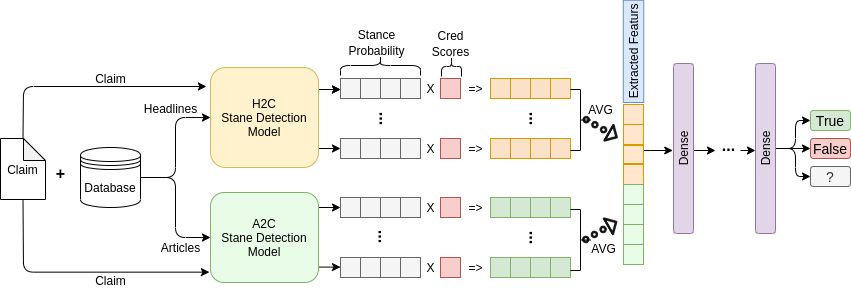
\includegraphics[width=14.5cm]{statistics/schema/fn.png} }
	\caption{Schematic of each fake news detection model.}%
	\label{fig:fnschm}%
\end{figure}

The credibility of news websites is one of the most important extracted features. The credibility can be calculated through the following steps (The credibility score of head-claim and article-claim is calculated similarly except using their related stance ground truth):

\begin{itemize}
	\item \textbf{Initialization}: The credibility score of all news websites that are existing in the \cite{stance_persian} dataset is set to zero at first. For the test set or predicting new samples, if the website doesn't exist in the data set, the credibility score is set to 0.1.


	\item \textbf{Quantification:}
	For each sample in the dataset, the credibility score changes according to Table \ref{tbl:cred}. $\rho$ value is calculated from equation \ref{eq:cred} if it is needed.
	\begin{table}[H]
		\centering
		\caption{Value of credibility according to GroundTruth and Veracity labels. }
		\setlength{\extrarowheight}{5pt}%
		\begin{tabular}{|l|l|l|}
			\hline
			GroundTruth & Veracity & Value \\
			\hline \hline
			Agree       & True     & $+1$    \\
			\hline
			Disagree    & False    & $+1$    \\
			\hline
			Agree       & False    & $-1$    \\
			\hline
			Disagree    & True     & $-1$    \\
			\hline
			Discuss     & True     & $+\rho$    \\
			\hline
			Discuss     & False    & $-\rho$   \\
			\hline
			Unrelated     & -   & No change   \\
			\hline
			-     & Discuss    & No change   \\
			\hline
		\end{tabular}
		\label{tbl:cred}
	\end{table}

	\begin{equation}
	\label{eq:cred}
	\rho = \frac{\text{P}(x,\text{Agree}) - \text{P}(x,\text{Disagree})}{\text{P}(x,\text{Agree}) + \text{P}(x,\text{Disagree})}\\
	\end{equation}

where: 
\begin{eqexpl}[25mm]
\item{$\text{P}(x,\text{Agree})$} Probability of Agree
\item{$\text{P}(x,\text{Disagree})$} Probability of Disagree 
\end{eqexpl}
	
	\item \textbf{Score Calculation:} The credibility score for each news website is calculated from equation \ref{eq:honesty}.
	\begin{equation}
	\label{eq:honesty}
	\text{H}(X) = \frac{\sum_{i=1}^{\text{k}_{X}} \text{credibility\,of\,}x_{i}}{\text{k}_{X}}
	\end{equation} 
	where:
	\begin{eqexpl}[25mm]
		\item{$\text{X}$} A news website
		\item{$\text{k}_{x}$} The number of news article in the dataset from x
		\item{$\text{credibility\,of\,}x_{i}$} Due to table \ref{tbl:cred}
	\end{eqexpl}

\end{itemize}


Also other features are extracted to detect fake news, such as :
\begin{itemize}
	\item One-hot encoding of the news website domain
	\item The ratio of samples that have been properly labeled as agree or disagree to the total sample of the news website (Correct ratio)
	\item The ratio of samples that have been wrongly labeled as agree or disagree to the total sample of the news website (Wrong ratio)
	\item The ratio of the total number of news website articles to the total number of articles in the data set.	
\end{itemize}



